%%%% Header %%%%%%%%%%%%%%%%%%%%%%%%%%%%%%%%%%%%%%%%%%%%%%%%%%%%%%%%%%%%%%%%%%%

\documentclass[
  12pt
]{scrartcl}

\usepackage{jonas}

\bibliography{/home/jon/lucile/share/jowncloud/sci/refs/refs.bib}
\hyphenation{}

%%%% Meta data %%%%%%%%%%%%%%%%%%%%%%%%%%%%%%%%%%%%%%%%%%%%%%%%%%%%%%%%%%%%%%%%

\usepackage[
  pdfauthor   ={Jonas Schöley},
  pdftitle    ={The Human Mortality Explorer},
  pdfsubject  ={Interactive Visualization},
  pdfkeywords ={visualization, R, shiny, mortality, hmd, Lexis surfaces},
  pdfproducer =Latex,
  pdfcreator  =pdflatex
]{hyperref}

\title{The Human Mortality Explorer}
\subtitle{An Interactive Online Visualization \vskip 0.2em of the Human Mortality Database}
\author{Jonas Schöley}

%%%% Titlepage %%%%%%%%%%%%%%%%%%%%%%%%%%%%%%%%%%%%%%%%%%%%%%%%%%%%%%%%%%%%%%%%

\begin{document}

\maketitle

\begin{center}
  {\Large\color{PineGreen} Please visit\\\url{https://jschoeley.shinyapps.io/hmdexp}\\to experience the \emph{Human Mortality Explorer}.}
\end{center}

\begin{figure}[ht!]
  \centering
  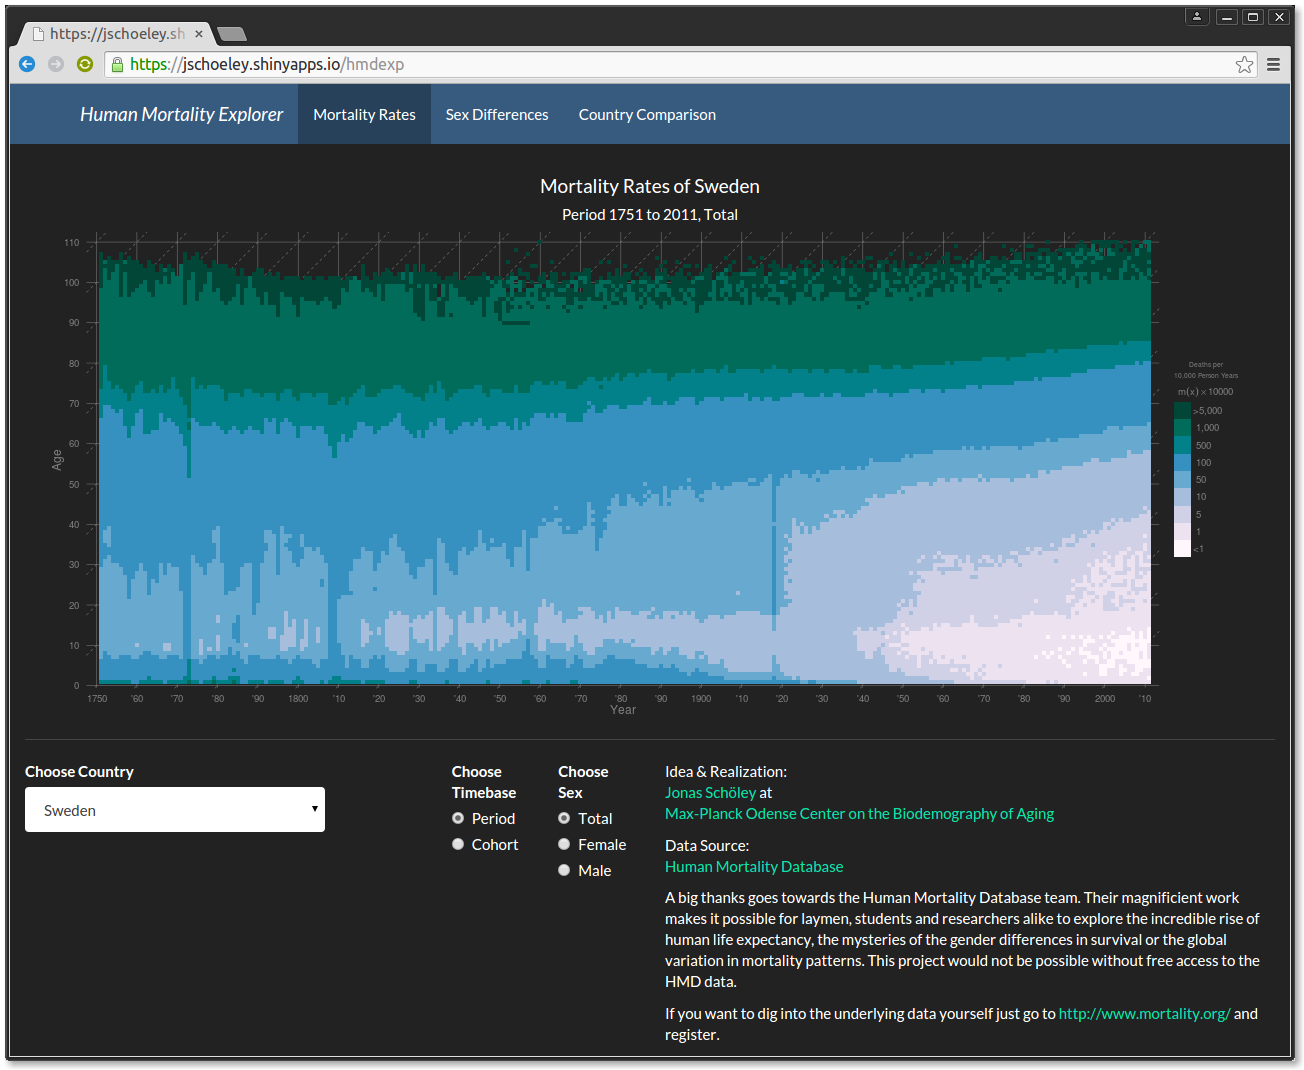
\includegraphics[width = 0.7\textwidth]{./fig/hmd_screen_mx.png}
  \caption{The Human Mortality Explorer: Mortality surface view.}
  \label{fig:mx}
\end{figure}

\begin{abstract2}
  The \emph{Human Mortality Explorer} is an interactive web page for the visual exploration of the Human Mortality Database. The tools allows users from all around the world to easily explore human mortality dynamics across space and time. Users select data subsets on a graphical user interface and are immediately presented with results in the form of Lexis surface plots (heatmaps over period and age). Users can toggle between a visualization of the pure mortality rates, sex differences in mortality and country comparisons. The Human Mortality Explorer is build using modern technologies that facilitate the construction of interactive web-pages without requiring expert knowledge on web-technologies.
\end{abstract2}

\clearpage

%%%% Text %%%%%%%%%%%%%%%%%%%%%%%%%%%%%%%%%%%%%%%%%%%%%%%%%%%%%%%%%%%%%%%%%%%%%

\section*{Background}

Interactive visualizations are the medium of many success stories in recent years. \enquote{The Global Flow of People} (\cite{Sander2014}), \enquote{Gapminder World} (\cite{Rosling2006}) or \enquote{What's Really Warming the World?} (\cite{Roston2015}) are a few examples of visualizations able to motivate people to explore data and to generate publicity for the underlying study or newspaper article. Less visible but equally important are domain specific visualization tools which help scientists with specific data analysis tasks such as genome analysis (\enquote{MizBee}, \cite{Meyer2009}), cluster analysis (\enquote{Hierarchical Clustering Explorer}, \cite{Seo2002}), browsing linguistic networks (\enquote{Constellation}, \cite{Munzner1999}), poetry analysis (\enquote{RhymeDesign}, \cite{McCurdy2015}) or investigative journalism (\enquote{RevEx}, \cite{Bertini2015}), to name a few.

Today the barrier of entry for building such applications is lower than ever and researchers can build web-based tools themselves without relying on external expertise. The \emph{Human Mortality Explorer}, a web application designed for easy exploration of the popular Human Mortality Database (\cite{Hmd2015}), serves to demonstrate this point. It has been developed over the course of a month by a single researcher.

\section*{Objective}

The objective is to develop a tool that allows for the easy and quick exploration of data on human mortality by researchers, students and interested laymen. Researchers should be able to quickly check existing hypotheses against the data and generate new ones. Teachers are given a tool to demonstrate human mortality patterns while being able to spontaneously explore the HMD data together with their students, facilitating classroom interactions. The interested public should have easy access to the tool (in terms of availability and ease-of-use) and be able to gain their own insights from the HMD data. A glossary of technical terms and interpretation guidelines allows non-demographers to use the tool.

\section*{Methods}

The application is written in the \texttt{R} language for statistical computing (\cite{RCT2014}). The \texttt{shiny} library (\cite{Chang2015}) is used to build a web-based user interface from within \texttt{R}. A special web server capable of interpreting \texttt{R + shiny} code hosts the application. The choice of tools illustrates an important point: Nowadays web-applications can be build by a single researcher, in a known programming environment, without deep knowledge about \texttt{HTML}, \texttt{Java Script} or other web technologies. Development takes place in the open. The source code is publicly available at an online repository (\url{https://github.com/jschoeley/hmdexp/}).

\section*{Contribution}

We contribute the \emph{Human Mortality Explorer}. An interactive web page for the visual exploration of the Human Mortality Database, visualizing death across time and space. The application is build around a heatmap representation of human mortality data on a Lexis surface (a period-age-grid). The user selects subsets of the data (country, sex, period or cohort rates) and is presented with the corresponding visualization. Currently there are three exploration views to choose from: pure mortality rates (see figure \ref{fig:mx}), sex differences of mortality rates (see figure \ref{fig:mx_sex_diff}) and country differences of mortality rates (see figure \ref{fig:mx_cntry_diff}).

The Human Mortality Explorer is in active development and not yet feature complete. Among other things, the final tool will feature:

\begin{compactenum}
  \item The visualization of HMD life-table data ($d_x, q_x, l_x, L_x, T_x, e_x$),
  \item the selection of a continuous colour scale,
  \item zooming into the graph,
  \item a glossary and interpretation guidelines.
\end{compactenum}

The project can be adopted for the Human Fertility Database (\cite{HFDT2015}) with little additional work, as both databases have similar data structures.

\begin{figure}[ht!]
  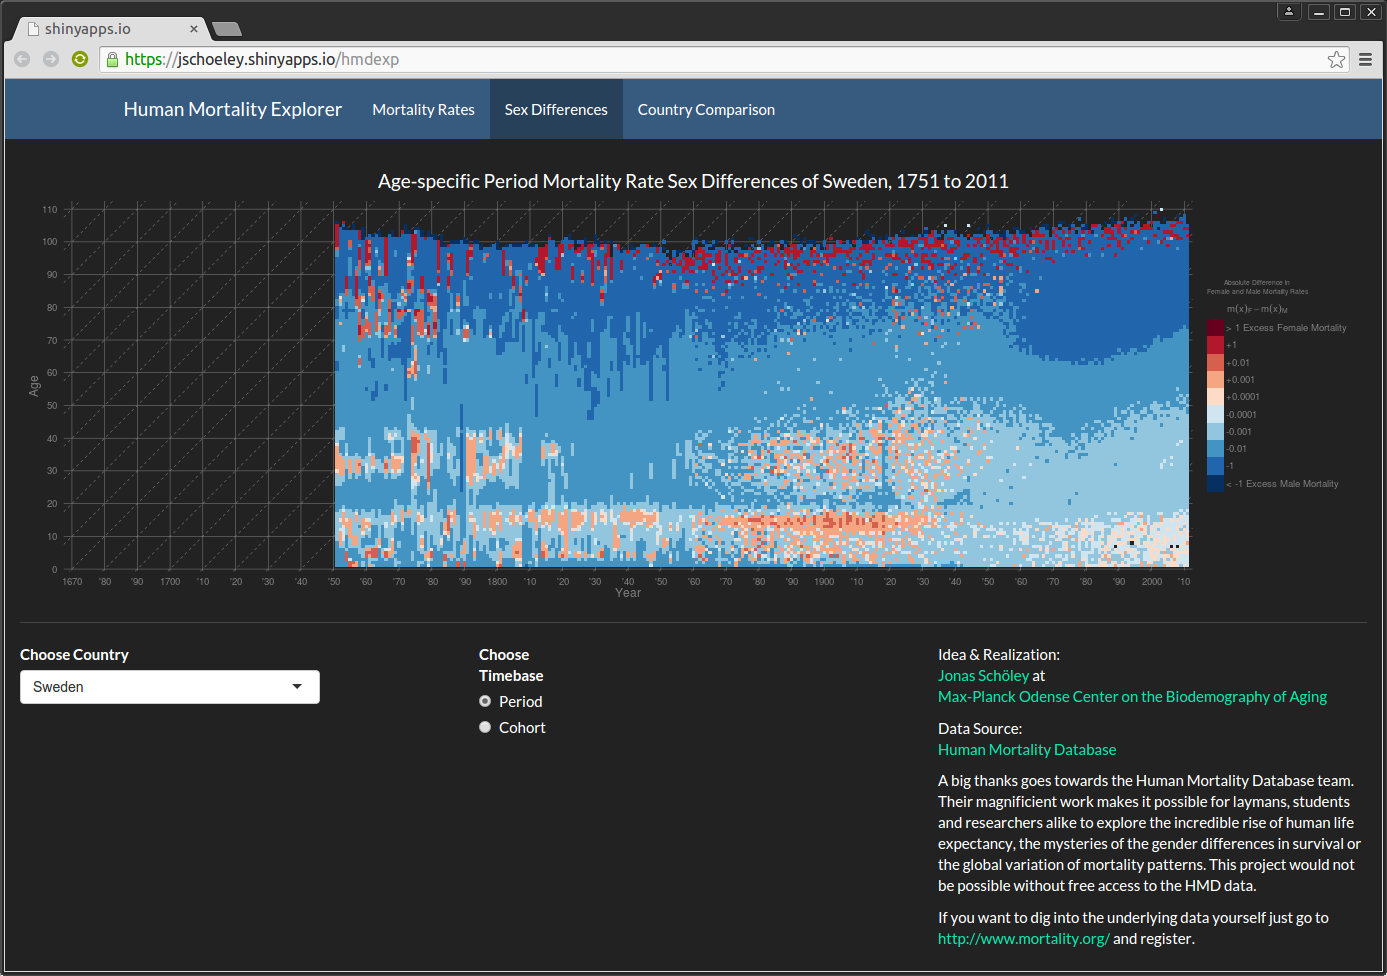
\includegraphics[width = \linewidth]{./fig/hmd_screen_mx_sex_diff.png}
  \caption{The Human Mortality Explorer: Sex differences view.}
  \label{fig:mx_sex_diff}
\end{figure}

\begin{figure}[ht!]
  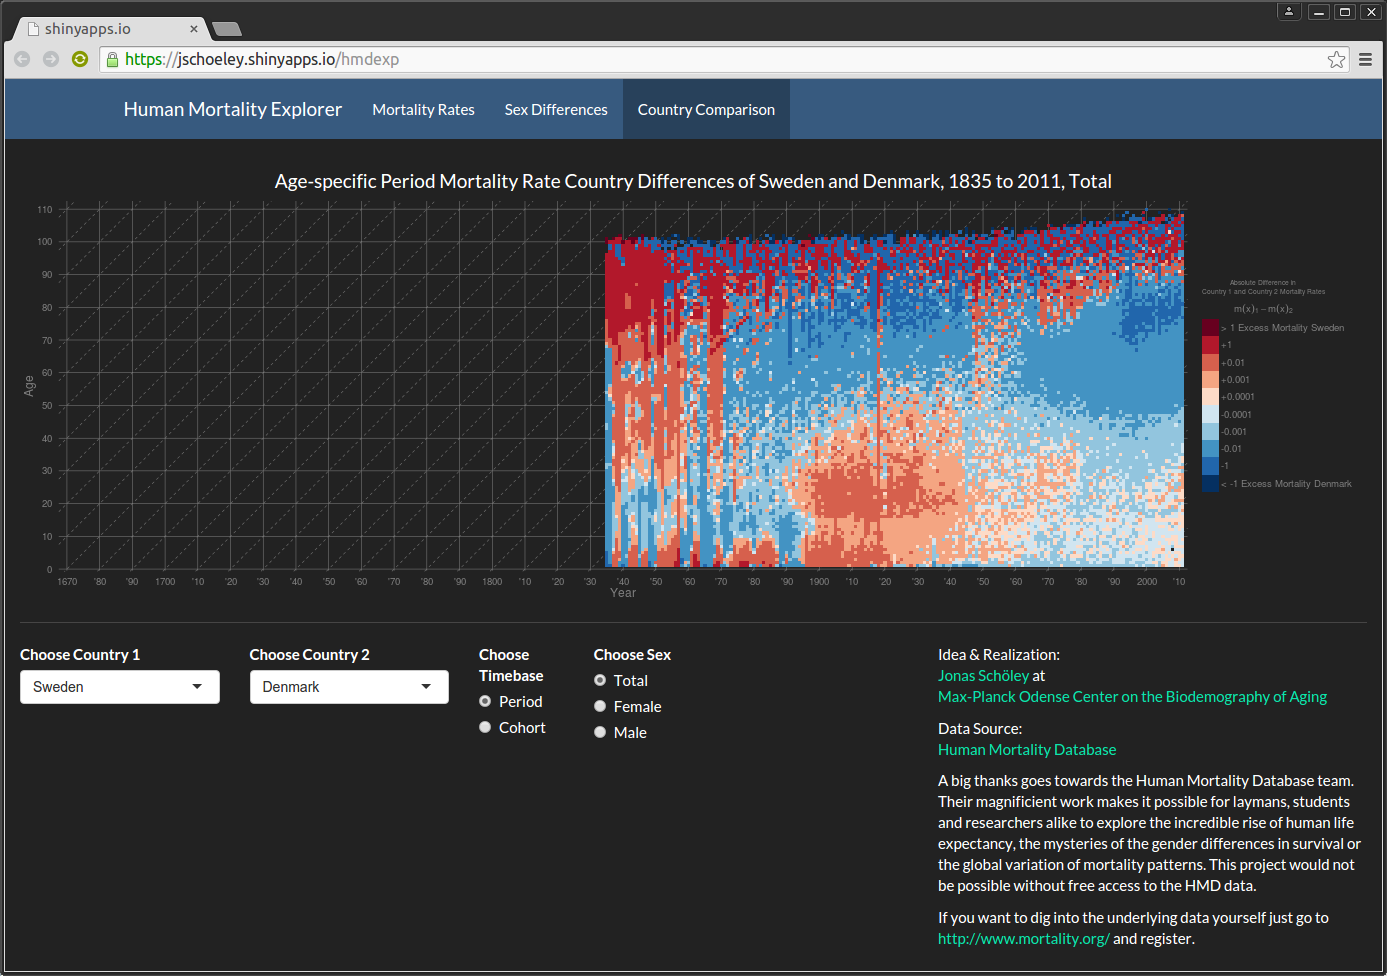
\includegraphics[width = \linewidth]{./fig/hmd_screen_mx_cntry_diff.png}
  \caption{The Human Mortality Explorer: Country comparison view.}
  \label{fig:mx_cntry_diff}
\end{figure}

\clearpage

%%%% Bibliography %%%%%%%%%%%%%%%%%%%%%%%%%%%%%%%%%%%%%%%%%%%%%%%%%%%%%%%%%%%%%

\sloppy
\printbibliography

%\clearpage

%%%% Appendix %%%%%%%%%%%%%%%%%%%%%%%%%%%%%%%%%%%%%%%%%%%%%%%%%%%%%%%%%%%%%%%%%

% appendix figures follow A1, A2, B1... scheme
%\renewcommand\thefigure{\thesection.\arabic{figure}}
%\setcounter{figure}{0}

%\begin{appendix}
%\end{appendix}

\end{document}